
    \chapter{Functional Requirements}
%\section{Functional Requirements}
    \begin{section}{Allow Student to Draw a Diagram}
        Description: Student given tools and space to draw an ER diagram \newline
        Primary Actor: Student \newline
        Precondition: Student is logged in and viewing a            question \newline
        Trigger: Student chooses a question to work on \newline
        Success end condition: Student can submit answer            \newline
        Failed end condition: Diagram is not drawn \newline
        \newline
        Steps:
        \begin{enumerate}
            \item{Empty space available to draw diagram}
            \item{Student picks a diagram type (Chen's/Crow's Foot)}
            \item{Student picks shapes from toolbox and places in           diagram}
            \item{Student places text inside shapes}
            \item{Student places links between shapes}
            \item{Student can edit or remove anything already placed on the diagram before finalizing}
        \end{enumerate}
        Exceptions:
        \begin{itemize}
            \item{Author draws diagram that students must edit             \newline
                Draw space will not be empty, student will be able to           make changes to present diagram}
        \end{itemize}
    \end{section}

    
    \begin{section}{Submit Answer}
        Description: Student submits answer to be checked and saved by the system \newline
        Primary Actor:Student \newline
        Precondition: Student is ready to submit answer \newline
        Trigger: Pressing the submit button \newline
        Success end condition: Feedback and/or grade is given       \newline
        Failed end condition: Nothing is given back to student      \newline
        \newline
        Steps:
        \begin{enumerate}
            \item{Student submits answer by pressing the submit             button}
            \item{System processes answer and decides validity*}
            \item{Outputs feedback and/or grade for student to see}
            \item{Answer is saved into database*}
        \end{enumerate}
        Exceptions:
        \begin{itemize}
            \item{Student leaves area blank \newline
        	Answer is just marked as wrong}
            \item{Author never properly input the correct answer or     feedback \newline
        	Student is told that there's nothing to report}
        \end{itemize}
    \end{section}

	
	%%%%%%%%%%%%%%%%%%%%%%%%%%%%%%%%%
    \begin{section}{Instructor logs in}
		Description: The Instructor is logging in, in order to access the Online Tutor System, using his/her NetID and password. \newline
		Primary Actor: Instructor \newline
		Precondition: The Instructor is on the login page of the system. \newline
		Trigger: The Instructor wants to log into the Online Tutor System. \newline
		Successful End Condition: The Instructor successfully logs into the Online Tutor System. \newline
		Failed End Condition: The Instructor is unable to log into the Online Tutor System. \newline
        \newline
        Steps:
        \begin{enumerate}
            \item{The Instructor enters his/her NetID in the username textfield.}
            \item{The Instructor enters his/her password in the password textfield.}
            \item{The Instructor clicks on the ‘login’ button to enter the system.}
        \end{enumerate}
        Exceptions:
        \begin{itemize}
            \item{The Instructor enters an incorrect NetID. In this case a message will be displayed that notifies that the NetID is incorrect.}
			\item{The Instructor enters an incorrect password. In this case a message will be displayed that notifies that the password is incorrect.}
        \end{itemize}
    \end{section}	
	
	%%%%%%%%%%%%%%%%%%%%%
    \begin{section}{Instructor creates new assignment*}
		Description: Instructor creates new assignment for students to be completed \newline
		Primary Actor: Instructor \newline
		Precondition: Instructor is logged in into tutoring system \newline
		Trigger: Instructor clicks on the create an assignment link \newline
		Successful End Condition(s): Assignment is added to the database and students are able to see it \newline
		Failed End Condition: No new assignment added \newline
        \newline
        Steps:
        \begin{enumerate}
            \item{Instructor clicks on the Create new assignment button on his homepage.}
            \item{Instructor chooses the class assignment is made for}
            \item{Instructor selects questions from database to be added to assignment}
            \item{Instructor names the assignment}
            \item{Instructor picks a deadline for the assignment}
            \item{Instructor clicks submit button}
            \item{Assignment is added to database}
        \end{enumerate}
        Exceptions:
        \begin{itemize}
            \item{An assignment with same name already exists.}
        \end{itemize}
    \end{section}


	%%%%%%%%%%%%%%%%%%%%%%%%%%%%%%%%%
    \begin{section}{Instructor Removes Assignment*}
		The Instructor will be removing an assignment from the assignment list. \newline
		Primary Actor: Instructor \newline
		Precondition: There must be at least one assignment in the database. \newline
		Trigger: Instructor selects to remove an assignment \newline
		Success end condition: The Instructor has successfully deleted an assignment \newline
		Failed end condition: The assignment list still shows the assignment that was supposed to be delete \newline
		\newline
        Steps:
        \begin{enumerate}
            \item{Instructor logs into system.}
            \item{Instructor selects remove assignment(s).}
            \item{The Instructor now has a list of assignments from which they can choose from.}
            \item{The Instructor selects one or more assignments to delete.}
			\item{Select delete assignment(s) and then the select assignments are deleted.}
        \end{enumerate}
        Exceptions:
        \begin{itemize}
            \item{None}
        \end{itemize}
    \end{section}		
	
	%%%%%%%%%%%%%%%%%%%%%%%%%%%%%%%%%%%%%%%
    \begin{section}{Instructor adds/removes question from the question bank to the assignment*}
		Description: Instructor adds or removes questions for an already created assignment \newline
		Primary Actor: Instructor \newline
		Precondition:  Instructor is logged in \newline
		Trigger: Instructor clicks on ''add/remove question'' button in the particular assignment \newline
		Successful End Condition: Question is added/removed from list of question for a particular assignment \newline
		Failed End Condition: Question that was added/removed is still in the list of questions for the assignment \newline
		\newline
        Steps:
        \begin{enumerate}
            \item{Instructor chooses assignment he wants to add/remove questions to from the list of already created assignments.}
            \item{Instructor clicks on “add/remove questions” button.}
            \item{Instructor can search the bank of questions that has been created by a type/topic of question.}
            \item{Instructor adds question he likes to the assignment.}
            \item{Instructor can remove any question he previously chosen from the list of questions.}
            \item{Instructor then click on submit button.}
			\item{List of question for that assignment is updated in the database.}
        \end{enumerate}
        Exceptions:
        \begin{itemize}
            \item{None.}
        \end{itemize}
    \end{section}
    
	%%%%%%%%%%%%%%%%%%%%%%%%%%%%%%%%%
    \begin{section}{Instructor views assignment}
		The Instructor will be viewing any assignment from the assignment list \newline
		Primary Actor: Instructor \newline
		Precondition: Instructor is logged into the system \newline
		Trigger: Instructor selects to view an assignment \newline
		Successful End Condition: Assignment is retrieved from database and can be viewed by the Instructor\newline
		Failed End Condition: Assignment failed to load \newline
        \newline
        Steps:
        \begin{enumerate}
            \item{Instructor selects view assignment.}
            \item{Instructor now has a list of assignments from which they can choose from.}
            \item{Instructor selects an assignment.}
            \item{Page will appear allowing the Instructor to view the assignment/questions.}
        \end{enumerate}
        Exceptions:
        \begin{itemize}
            \item{None.}
        \end{itemize}
    \end{section}	
	
	%%%%%%%%%%%%%%%%%%%%%%%%%%%%%%%%%
    \begin{section}{Instructor views Student reports}
		The Instructor wants to view any student's report for any assignment that the student attempted. \newline
		Primary Actor: Instructor \newline
		Precondition: Student has attempted the assigned questions \newline
		Trigger: Instructor attempts to view students stats \newline
		Successful End Condition: Students scores are retrieved and displayed on the report page \newline
		Failed End Condition: Student report failed to load \newline
		\newline
        Steps:
        \begin{enumerate}
            \item{Instructor selects to view assignments list.}
            \item{Instructor selects assignments.}
            \item{System sends statistics of the class of the select assignment (overall average class attempts, average grade, median grade, highest grade, lowest grade, etc).}
            \item{Instructor can select to click on individual student statistics of the assignment.}
			\item{System displays statistic of individual student for the select assignment.}
        \end{enumerate}
        Exceptions:
        \begin{itemize}
            \item{No students were signed up for assignment.}
			\item{No assignments have been created yet.}
        \end{itemize}
                        \begin{figure}[H]
            \centerline{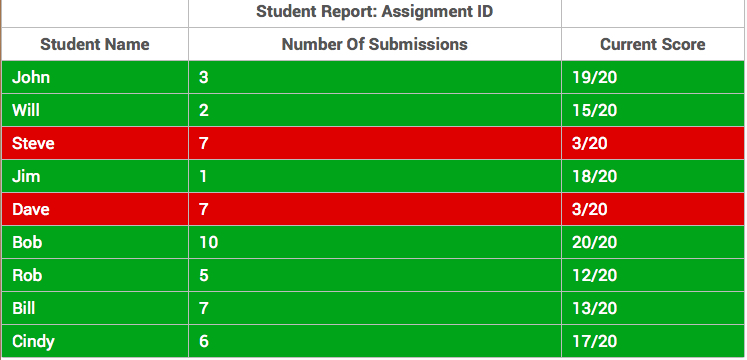
\includegraphics[height=7cm]{StudentReport.jpg}}
            \caption{The students report that is displayed to the Instructor}
    \end{figure}
    \end{section}	
	

	

	
	
	%%%%%%%%%%%%%%%%%%%%%%%%%%%%%%%%%
    \begin{section}{User registers for the Online Tutor System}
		Description: An author, student, or instructor registers for the Online Tutor System. \newline
		Primary Actor: User \newline
		Precondition: The user has navigated to the website of the Online Tutor System. \newline
		Trigger: The user clicks the button to register for the Online Tutor System. \newline
		Successful End Condition: The user is successfully registered and provided access to the Online Tutor System. \newline
		Failed End Condition: The user is not successfully registered and does not have access to the Online Tutor System. \newline
		\newline
        Steps:
        \begin{enumerate}
            \item{The user fills in his/her NetID.}
            \item{The user fills in his/her password corresponding with his/her NetID.}
            \item{The NetID and password are the same NetID and password as registered at the University of Massachussetts.}
			\item{The user clicks the ‘register’ button.}
			\item{The user is registered in the Online Tutor System.}
			\item{The user is redirected to his/her homepage (which varies based on type of user).}
        \end{enumerate}
        Exceptions:
        \begin{itemize}
            \item{The user enters an incorrect NetID that is not registered at the University of Massachusetts. In this case a message will be displayed that notifies that the NetID is incorrect.}
			\item{The user enters a password that does not correspond to the NetID that is registered at the University of Massachusetts. In this case a message will be displayed that notifies that the password is incorrect..}
        \end{itemize}
    \end{section}		
	
        
    \begin{section}{Student Logs In}
        Description: The student is logging in, in order to access the tutor system using their NetID and password. \newline
        Primary Actor: Student \newline
        Secondary Actor: System \newline
        Precondition: The student is on the login page of the system. \newline
        Trigger: The student wants to log into the tutoring system. \newline
        Successful End Condition: The student successfully logs into the tutoring system. \newline
        Failed End Condition:  The student is unable to log into the system \newline
        \newline
        Steps:
        \begin{enumerate}
            \item{The student enters their NetID in the username textbox}
            \item{The student enters their password in the password textbox}
            \item{The student clicks on the LOGIN button to enter the system}
        \end{enumerate}
        Exceptions:
        \begin{itemize}
            \item{If the student does not enter the correct NetID or password the system will 
            not log the student in and a message will appear stating that the NetID or password 
            that they entered is incorrect and to please try again.}
        \end{itemize}
    \end{section}
    
    \begin{section}{Student Selects an Assignment}
        Description: Once logged in, the student can view any available assignment \newline
        Primary Actor: Student \newline
        Precondition: Student is already logged in \newline
        Trigger: Student logs in \newline
        Successful End Condition: Student can view all questions in an assignment \newline
        Failed End Condition: Student is unable to see any questions in the assignment \newline
        \newline
        Steps:
        \begin{enumerate}
            \item{Student clicks on desired assignment}
            \item{Student can select any of the question(s) in the assignment}
            \item{Student can go back to home page and select any other assignment}
        \end{enumerate}
        Exceptions:
        \begin{itemize}
            \item{There are no assignments available, student has nothing to view.}
        \end{itemize}
            \begin{figure}[H]
            \centerline{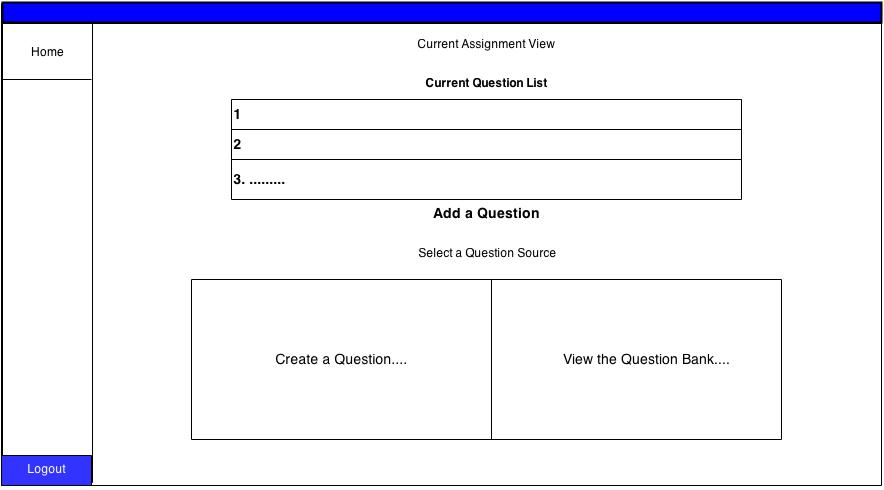
\includegraphics[height=7cm]{AssignmentView.jpg}}
            \caption{Assignment View from the student's perspective}
    \end{figure}
    \end{section}
    
    \begin{section}{Student Selects Question to Answer}
        Description: Student views a question that he would like to answer \newline
        Primary Actor: Student \newline
        Precondition: Student is logged in and is in an assignment         \newline
        Trigger: The student attempts to select a new question      to attempt to answer \newline
        Success End Condition: Question that the student selects     successfully loads \newline
        Failed End Condition: The question that is selected does     not load \newline
        \newline
        Steps:
        \begin{enumerate}
            \item{Student scrolls through the list of questions in the assignment.}
            \item{Student selects the question they would like to        answer from the list.}
            \item{Webpage for the selected question loads}
            \item{Student can view and answer question}
        \end{enumerate}
        Exceptions: None
    \end{section}
    
    
    \begin{section}{Student Views Question}
        Description: The student views a question that is part of an assignment. \newline
        Primary Actor: Student \newline
        Secondary Actor: System \newline
        Precondition: The student is logged into the system. \newline
        Trigger: The student clicks on the question to view it. \newline
        Successful End Condition: The student views the question they have selected. \newline
        Failed End Condition: The student is unable to view the question. \newline
        \newline
        Steps:
        \begin{enumerate}
            \item{The student selects an assignment to view.}
            \item{The student then selects a specific question to view.}
            \item{The student views the question.}
        \end{enumerate}
        Exceptions: None
        
                    \begin{figure}[H]
            \centerline{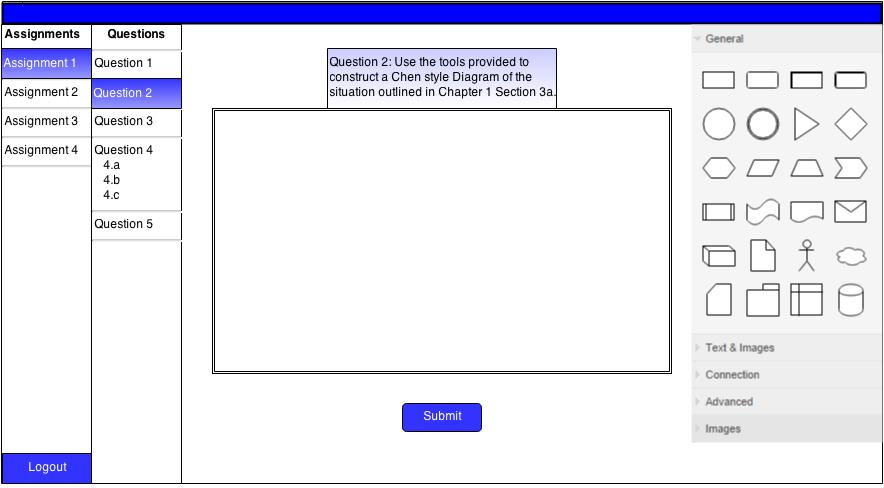
\includegraphics[height=7cm]{StudentQuestion.jpg}}
            \caption{Assignment View from the student's perspective}
    \end{figure}
        
    \end{section}

    
    \begin{section}{Student Submits Answer}
    Primary Actor: Student\\
    Precondition: Student has previously answered the question that he/she wants to submit.\\
    Trigger: Student wants to submit a question.\\
    Successful End Condition:Question is submited.\\
    Failed End Condition: Student does not submit the question.\\
    Steps:
    \begin{enumerate}
    \item Student clicks on submit.
    \item Student sees a feedback for the question he answered.
    \end{enumerate}
    Exceptions:
    \begin{itemize}
    
    \item Internet goes offline while the student is submitting the question.
    \item Student gets the wrong feedback
    
    \end{itemize}
    \end{section}
    

    
    \begin{section}{Student Views Feedback}
        Description: After submitting the question the student is able to see the feedback that is given for the 
        question based on if they answered the question correctly or not. \newline
        Primary Actor: Student \newline
        Secondary Actor: System \newline
        Precondition: The student has selected a question and answered the question. \newline
        Trigger: The student submits the answer to the question. \newline
        Successful End Condition: Feedback is displayed on the screen for the student 
        to read and use to help make their answer correct if it is incorrect. \newline
        Failed End Condition: There is no feedback that gets displayed. \newline
        \newline
        Steps:
        \begin{enumerate}
            \item{Once the answer has been submitted the system compares it to the correct answer given.}
            \item{If the answer is correct the question page displays the feedback that is 
            written by the author for a correct answer such as good job or correct.}
            \item{If the answer is incorrect the question page displays the feedback that is 
            written by the author for an incorrect answer such as a hint or common mistake.}
            \item{The student reads the feedback that is displayed on the screen.}
        \end{enumerate}
        Exceptions:
        \begin{itemize}
            \item{The author does not enter in any feedback for correct answers so no feedback will be displayed.}
            \item{The author does not enter in any feedback for incorrect answers so no feedback will be displayed.}
        \end{itemize}
                

    \end{section}
        
    \begin{section}{Author Logs In}
        Description: The author is logging in, in order to access the tutor system using their NetID and password. \newline
        Primary Actor: Author \newline
        Secondary Actor: System \newline
        Precondition: The author is on the login page of the system. \newline
        Trigger: The author wants to log into the tutoring system. \newline
        Successful End Condition: The author successfully logs into the tutoring system. \newline
        Failed End Condition:  The author is unable to log into the system because of an incorrect NetID or password or both \newline
        \newline
        Steps:
        \begin{enumerate}
            \item{The author enters his NetID in the username textbox}
            \item{The author enters his password in the password textbox}
            \item{The author clicks on the LOGIN button to enter the system}
        \end{enumerate}
        Exceptions:
        \begin{itemize}
            \item{If the author does not enter the correct NetID or password 
            the system will not log the student in and a message will appear stating 
            that the NetID or password that they entered is incorrect and to please try again.}
        \end{itemize}
    \end{section}
  
  
    
    \begin{section}{Author Views the Question Bank}
    
Description: The author views the questions that have already been created and are in the question bank.\\
Primary Actor: Author\\
Secondary Actor: System \\
Precondition: Author is logged in and there are questions in the question bank.\\
Trigger: The author would like to view the question bank.\\
Steps:
\begin{enumerate}
\item The author selects the questions tab.
\item The author is now viewing the question bank.

\end{enumerate}

Successful End Condition: The author is able to view the question bank.\\
Failed End Condition: The author is unable to view the question bank.\\
Exceptions:
\begin{itemize}
\item There are no questions in the question bank to view. The author sees an empty question bank.
\end{itemize}
    \begin{figure}[H]
            \centerline{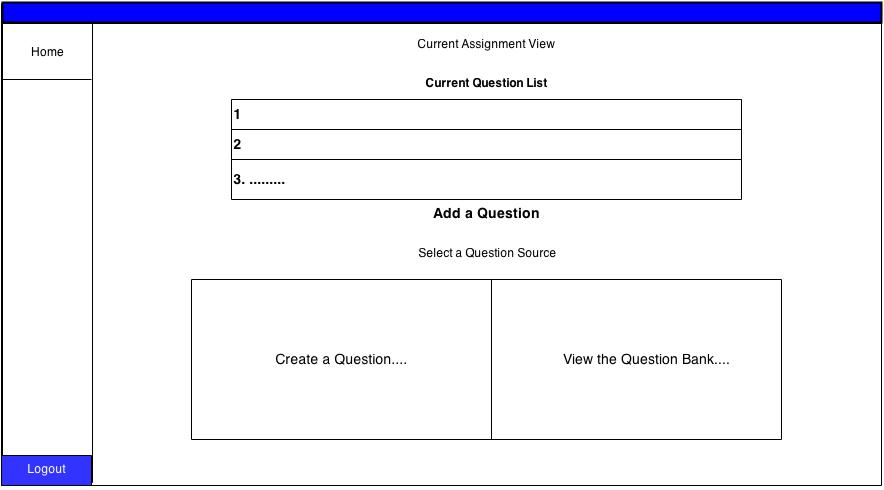
\includegraphics[height=7cm]{AssignmentView.jpg}}
            \caption{View Question Bank Diagram}
    \end{figure}
    \end{section}
    
    
    
    \begin{section}{Author Adds a New Question to Question Bank}
      Description: Author adds a new question to the question bank. \newline
        Primary Actor: Author.  \newline
        Secondary Actor: System  \newline
        Precondition: Author is logged into the Online Tutor System. \newline
        Trigger: The author would like to add a new question to the question bank. \newline
        Successful End Condition: A question is successfully added to the question Bank. \newline
        Failed End Condition: The question is not added to the question bank.
   \newline
        \newline
        Steps:
        \begin{enumerate}
            \item{Author goes to question bank section.}
            \item{Author clicks on ''Add'' button to add a question.}
            \item{Author input the question in a textbox.}
		\item{Author provides the appropriate feedback to the question.}
		\item{Author clicks on a ''Submit'' button.}
        \end{enumerate}
        Exceptions:
        \begin{itemize}
            \item{Author submits wrong feedback.}
	    \item{Internet goes offline while author was writing the question and/or feedback.}
        \end{itemize}
        
                \begin{figure}[H]
            \centerline{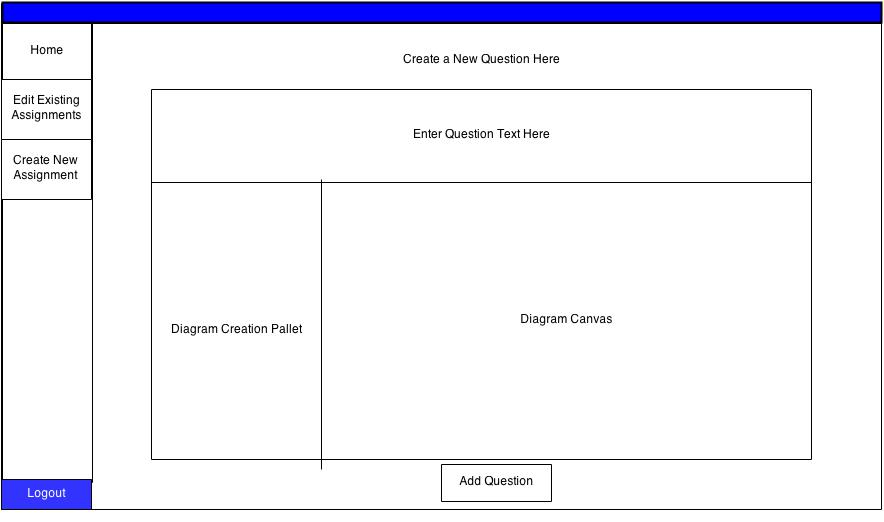
\includegraphics[height=7cm]{Add.jpg}}
            \caption{Add-Question UI}
    \end{figure}
    \end{section}
    
    
    
    \begin{section}{Author Edits a Question From the Question Bank}
        Description: The author wants to edit a question that is already in the question bank by changing any or all of the different parts of the question. \\
        Primary Actor: Author \\
        Secondary Actor: System \\
        Precondition: The author has already created the question that he/she wishes to edit. \\
        Trigger: The author is viewing a question that he/she wishes to edit. \\
        Successful End Condition: The question changes have been made and the author is prompted that his/her changes have been made. \\
        Failed End Condition: The question does not get updated and the author is prompted saying that the question was not changed. \\
        \\
        Steps:
        \begin{enumerate}
            \item{The author selects the edit button.}
            \item{The author edits the question text.}
            \item{The author edits the question correct answer.}
            \item{The author edits the question feedback.}
            \item{The author saves the changes to the question and answer.}
        \end{enumerate}
        Exceptions:
        \begin{itemize}
            \item{The author does not want to edit the question text so they do not edit it and leave it alone.}
            \item{The author does not want to edit the question correct answer so they do not edit it and leave it alone.}
            \item{The author does not want to edit the question feedback so they do not edit it and leave it alone.}
            \item{The author does not save the changes to the question so the changes are not saved.}
            \item{The author exits the system without saving the changes to the questions resulting in none of the changes being saved.}
        \end{itemize}
    \end{section}
    
    
    \begin{section}{Author Removes a Question From the Question Bank}
    Description: The author views the questions that have already been created and are in the question bank. \\
        Primary Actor: Author.  \\
        Secondary Actor: System. \\
        Precondition: Author is logged in and there are questions in the question bank.\\
        Trigger: The author would like to remove a question from the question bank. \\
        Successful End Condition:  The question is removed. \\
        Failed End Condition: The question is unable to be removed.\\
        \newline
        Steps:
        \begin{enumerate}
            \item{The author selects the questions tab to view the question bank.}
            \item{The author selects the specific question that they would like to remove.}
            \item{The author presses remove question.}
        \end{enumerate}
        Exceptions:
        \begin{itemize}
            \item{The question bank is empty and therefore the author is unable to remove any questions.}
        \end{itemize}
    \end{section}
    
    
    \begin{section}{Author Views a Question}
        Description: The author views a question that has been created. \newline
        Primary Actor: Author \newline
        Secondary Actor: System \newline
        Precondition: The author is logged into the system. \newline
        Trigger: The author would like to view a question. \newline
        Successful End Condition: The author views the question that they would like to view. \newline
        Failed End Condition: The author is unable to view the question that they want to view. \newline
        \newline
        Steps:
        \begin{enumerate}
            \item{The author selects the questions tab from their view.}
            \item{The author then scrolls through the list of questions.}
            \item{The author then selects the question they would like to view.}
            \item{The author then views the question.}
        \end{enumerate}
        Exceptions: None
    \end{section}
    
    
    \begin{section}{Author Copies a Question*} 
  
Description: The author takes an existing question and copies it creating a new question.\\
Primary Actor: Author\\
Secondary Actor: System\\
Precondition: The author is logged in and there is a question to copy.\\
Trigger: The author wants to copy a question.\\
Steps:
\begin{enumerate}
\item The author selects the questions tab to view the question bank.
\item They select the question which they would like to copy.
\item They choose to copy the question.
\item They make any necessary edits and then save the question.
\item The question is successfully copied.
\end{enumerate}
Successful End Condition: The copies a previously made question and is able to create a new one.\\
Failed End Condition: The author is unable to successfully copy a question.
Exceptions: 
\begin{itemize}
\item There are no questions in the question bank to copy.
\item They make no edits to the copied question and copy it as is.

\end{itemize}


    \end{section}

